\subsection{Activities}
\begin{frame}
  \frametitle{Activities}
  \fontsize{11}{10}\selectfont
  \begin{itemize}
  \item Activities are a single screen of the user interface of an
    application
  \item They are assembled to provide a consistent interface. If we
    take the example of an email application, we will have:
    \begin{itemize}
    \item An activity listing the received mails
    \item An activity to compose a new mail
    \item An activity to read a mail
    \end{itemize}
  \item Other applications might need one of these activities. To
    continue with this example, the Camera application might want to
    start the composing activity to share the just-shot picture
  \item It is up to the application developer to advertise available
    activities to the system
  \item When an activity starts a new activity, the latter replaces
    the former on the screen and is pushed on the \emph{back stack}
    which holds the last used activities, so when the user is done
    with the newer activity, it can easily go back to the previous one
  \end{itemize}
\end{frame}

\begin{frame}
  \frametitle{Back Stack}
  \begin{figure}[h!]
    \centering
    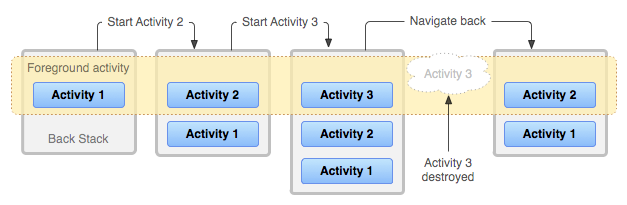
\includegraphics[width=\textwidth]{slides/android-application-activities/activity-backstack.png}\\
    {
      \tiny
      Credits: \url{http://developer.android.com}
    }
  \end{figure}
\end{frame}

\begin{frame}
  \frametitle{Back Stack}
  \begin{figure}[h!]
    \centering
    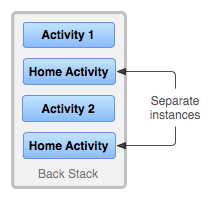
\includegraphics[height=0.65\textheight]{slides/android-application-activities/activity-backstack-instances.png}
    {
      \tiny
      Credits: \url{http://developer.android.com}
    }
  \end{figure}
\end{frame}

\begin{frame}
  \frametitle{Activity Lifecycle 1/3}
  \begin{itemize}
  \item As there is no single entry point and as the system manages
    the activities, activities have to define callbacks that the
    system can call at some point in time
  \item Activities can be in one of the three states on Android
    \begin{description}
    \item[Running] The activity is on the foreground and has focus
    \item[Paused] The activity is still visible on the screen but no
      longer has focus. It can be destroyed by the system under very
      heavy memory pressure
    \item[Stopped] The activity is no longer visible on the screen. It
      can be killed at any time by the system
    \end{description}
  \end{itemize}
\end{frame}

\begin{frame}
  \frametitle{Activity Lifecycle 2/3}
  \begin{itemize}
  \item There are callbacks for every change from one of these states
    to another
  \item The most important ones are \code{onCreate} and \code{onPause}
  \item All components of an application run in the same thread. If
    you do long operations in the callbacks, you will block the entire
    application (UI included). You should always use threads for every
    long-running task.
  \end{itemize}
\end{frame}

\begin{frame}
  \frametitle{Activity Lifecycle 3/3}
  \begin{figure}[h!]
    \centering
    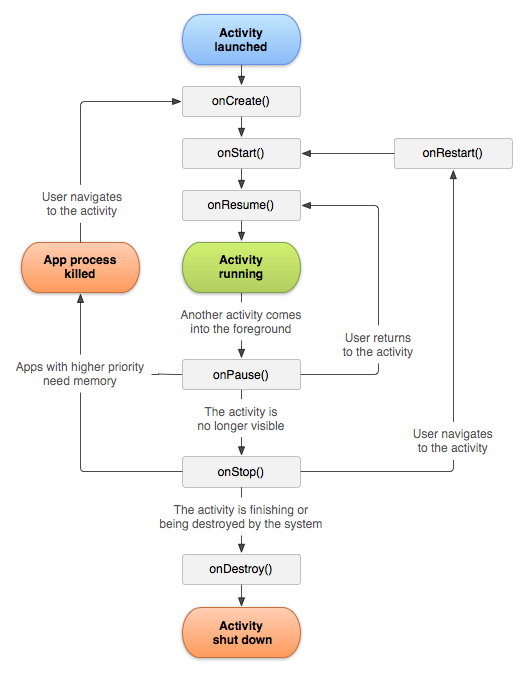
\includegraphics[height=0.8\textheight]{slides/android-application-activities/activity-lifecycle.png}\\
    {
      \tiny
      Credits: \url{http://developer.android.com}
    }
  \end{figure}
\end{frame}

\begin{frame}
  \frametitle{Saving Activity State 1/2}
  \begin{itemize}
  \item As applications tend to be killed and restarted quite often,
    we need a way to store our internal state when killed and reload
    it when restarted
  \item Once again, this is done through callbacks
  \item Before killing the application, the system calls the
    \code{onSaveInstanceState} callback and when restarting it, it
    calls \code{onRestoreInstanceState}
  \item In both cases, it provides a Bundle as argument to allow the
    activity to store what's needed and reload it later, with little
    overhead
  \end{itemize}
\end{frame}

\begin{frame}
  \frametitle{Saving Activity State 2/2}
  \begin{itemize}
  \item This make the creation/suppression of activities flawless for
    the user, while allowing to save as much memory as we need
  \item These callbacks are not always called though. If the activity
    is killed because the user left it in a permanent way (through the
    back button), it won't be called
  \item By default, these activities are also called when rotating the device,
    because the activity will be killed and restarted by the system to
    load new resources
  \end{itemize}
\end{frame}

\begin{frame}
  \frametitle{Activity Lifecycle}
  \begin{figure}[h!]
    \centering
    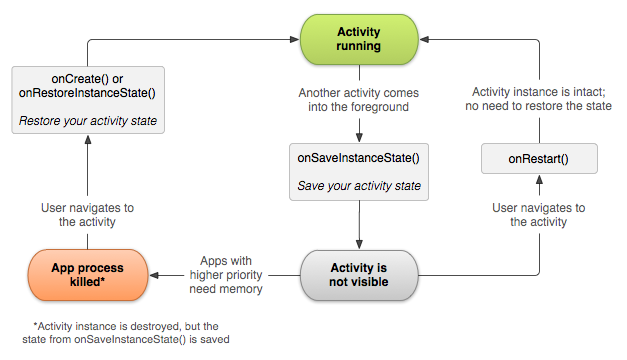
\includegraphics[width=\textwidth]{slides/android-application-activities/activity-saving.png}\\
    {
      \tiny
      Credits: \url{http://developer.android.com}
    }
  \end{figure}
\end{frame}

\begin{frame}
  \frametitle{Activity Callbacks}
  \begin{figure}[h!]
    \centering
    \includegraphics[width=\textwidth]{slides/android-application-activities/activity-callbacks.pdf}\\
    {
      \tiny
      Credits: \url{http://developer.android.com}
    }
  \end{figure}
\end{frame}

\begin{frame}[fragile]
  \frametitle{Activity HelloWorld}
\begin{minted}[fontsize=\scriptsize]{java}
public class ExampleActivity extends Activity {
    public void onCreate(Bundle savedInstanceState) {
        super.onCreate(savedInstanceState);
        setContentView(R.layout.example);
        Log.i("ExampleActivity", "Activity created!");
    }
    protected void onStart() {
        super.onStart();
    }
    protected void onResume() {
        super.onResume();
    }
    protected void onPause() {
        super.onPause();
    }
    protected void onStop() {
        super.onStop();
    }
    protected void onDestroy() {
        super.onDestroy();
    }
}
\end{minted}
\end{frame}
